%==============================================================================
% Sjabloon poster bachproef
%==============================================================================
% Gebaseerd op document class `a0poster' door Gerlinde Kettl en Matthias Weiser
% Aangepast voor gebruik aan HOGENT door Jens Buysse en Bert Van Vreckem

\documentclass[a0,portrait]{hogent-poster}

% Info over de opleiding
\course{Bachelorproef}
\studyprogramme{toegepaste informatica}
\academicyear{2022-2023}
\institution{Hogeschool Gent, Valentin Vaerwyckweg 1, 9000 Gent}

% Info over de bachelorproef
\title{Het performantie verschil tussen een REST API en een gRPC API bij het versturen van datasets}
\author{Nicolas Thiers}
\email{nicolas.thiers@student.hogent.be}
\supervisor{Benjamin Vertonghen}
\cosupervisor{Maarten Vandeperre (Viae Solutions)}

% Indien ingevuld, wordt deze informatie toegevoegd aan het einde van de
% abstract. Zet in commentaar als je dit niet wilt.
\specialisation{Mobile \& Enterprise development}
\keywords{gRPC; RPC; REST; API; Performantie}
\projectrepo{https://github.com/thiersnicolas/latex-hogent-bachproef-NT, https://github.com/thiersnicolas/gRPC_vs_REST}

\begin{document}

\maketitle

\begin{abstract}
  In dit onderzoek wordt het performantie verschil tussen een REST API en een gRPC API beschouwd bij het versturen van datasets van vari\"erende grootte.
  Beide technologie\"en zijn API's en daarmee helpen zij de communicatie tussen twee applicaties via HTTP te faciliteren. gRPC is een tamelijk recente ontwikkeling die
  dankzij een speciaal serialisatie- en compressie proces zeer performant zou moeten zijn. De vraag rijst dan in welke mate het sneller zou zijn dan REST en of het dat
  in alle omstandigheden is. Uit de performantie metingen van dit onderzoek blijkt dat gRPC niet noodzakelijk sneller is dan REST.
  Rekening houdend met andere verschillen tussen beide type API, waaronder ondersteuning door browsers, adoptie en flexibiliteit, lijkt dit een negatieve impact te
  hebben op het aantal scenario's waarbij er voor gRPC zou geopteerd worden.

\end{abstract}

\begin{multicols}{2} % This is how many columns your poster will be broken into, a portrait poster is generally split into 2 columns

\section{Inleiding}

In dit onderzoek wordt een Representational state transfer, REST, API vergeleken met een Remote Procedure Call, RPC, API, meer specifiek de
implementatie van Google nl. gRPC.
API staat voor Application programming interfaces en is een software-interface die het mogelijk maakt voor twee applicaties om met elkaar gegevens uit te wisselen.
Bij REST kan nog steeds het HTTP 1.1 protocol gebruikt worden terwijl gRPC enkel via het performantere HTTP 2 communiceert.
gRPC gebruikt echter specifieke delen van het HTTP 2 protocol waar moderne browsers geen ondersteuning voor bieden,
waardoor voor dergelijke communicatie een extra proxy moet voorzien worden.
gRPC serialiseert en comprimeert alle data d.m.v. protocol buffers waardoor het, op vlak van performantie, een overwicht zou verkrijgen t.a.v. REST.
Bij REST wordt data voornamelijk als JSON verzonden, wat meer uitvoerig is dan de geserialiseerde data via gRPC.
Er is echter geen verplichting voor een specifiek formaat waardoor bij REST data eventueel ook gecomprimeerd kan worden.
In tegenstelling tot gRPC is het gebruik van REST wijdverspreid en zijn er voldoende softwareontwikkelaars met kennis ter zake om een REST API vlot te implementeren.
Voor beide API's is het nodig een betrouwbaar en duidelijk contract aan te bieden aan een eventuele client.
Voor REST zijn er reeds veel oplossingen die een API documenteren en eventueel zelfs code genereren.
Bij gRP dient er een .proto bestand uitgewisseld te worden tussen server en client waarmee de nodige code door protocol buffers gegenereerd kan worden.\\
Elke softwareontwikkelaar of applicatie-architect dient bij de implementatie van een applicatie te evalueren wat de concrete noodzaken
zijn, en te overwegen welke technologie\"en daar het beste een oplossing voor bieden. Performantie is daarbij
steeds een belangrijke en vaak een doorslaggevende factor.

\section{Methodologie}

Voor het onderzoek worden een client en provider applicatie voorzien.
Beiden krijgen 2 rest implementaties, één dat data als JSON verzendt en het andere dat data nog comprimeert.
Ook zijn er 2 gRPC implementaties, het eerste zal de te verzenden data met protocol buffers serialiseren en daarna verzenden en het tweede,
ten volle gebruik makend van HTTP 2 functionaliteit, geeft de geserialiseerde data middels een stream door.
De server applicatie zal gehost worden op OpenShift van RedHat terwijl de client applicatie deze vanop een pc aanspreekt.
Tijdens de performantie-testen wordt het tijdsverloop geregistreerd bij aanvang van het aanroepen van de server door de client
tot de gevraagde data bij de client toekomt en gedeserialiseerd is. Dit proces wordt voor verschillende datasets herhaald.
Ook worden grotere datasets in stukken verzonden om het verschil in performantie te beschouwen.\\

\begin{center}
  \captionsetup{type=figure}
  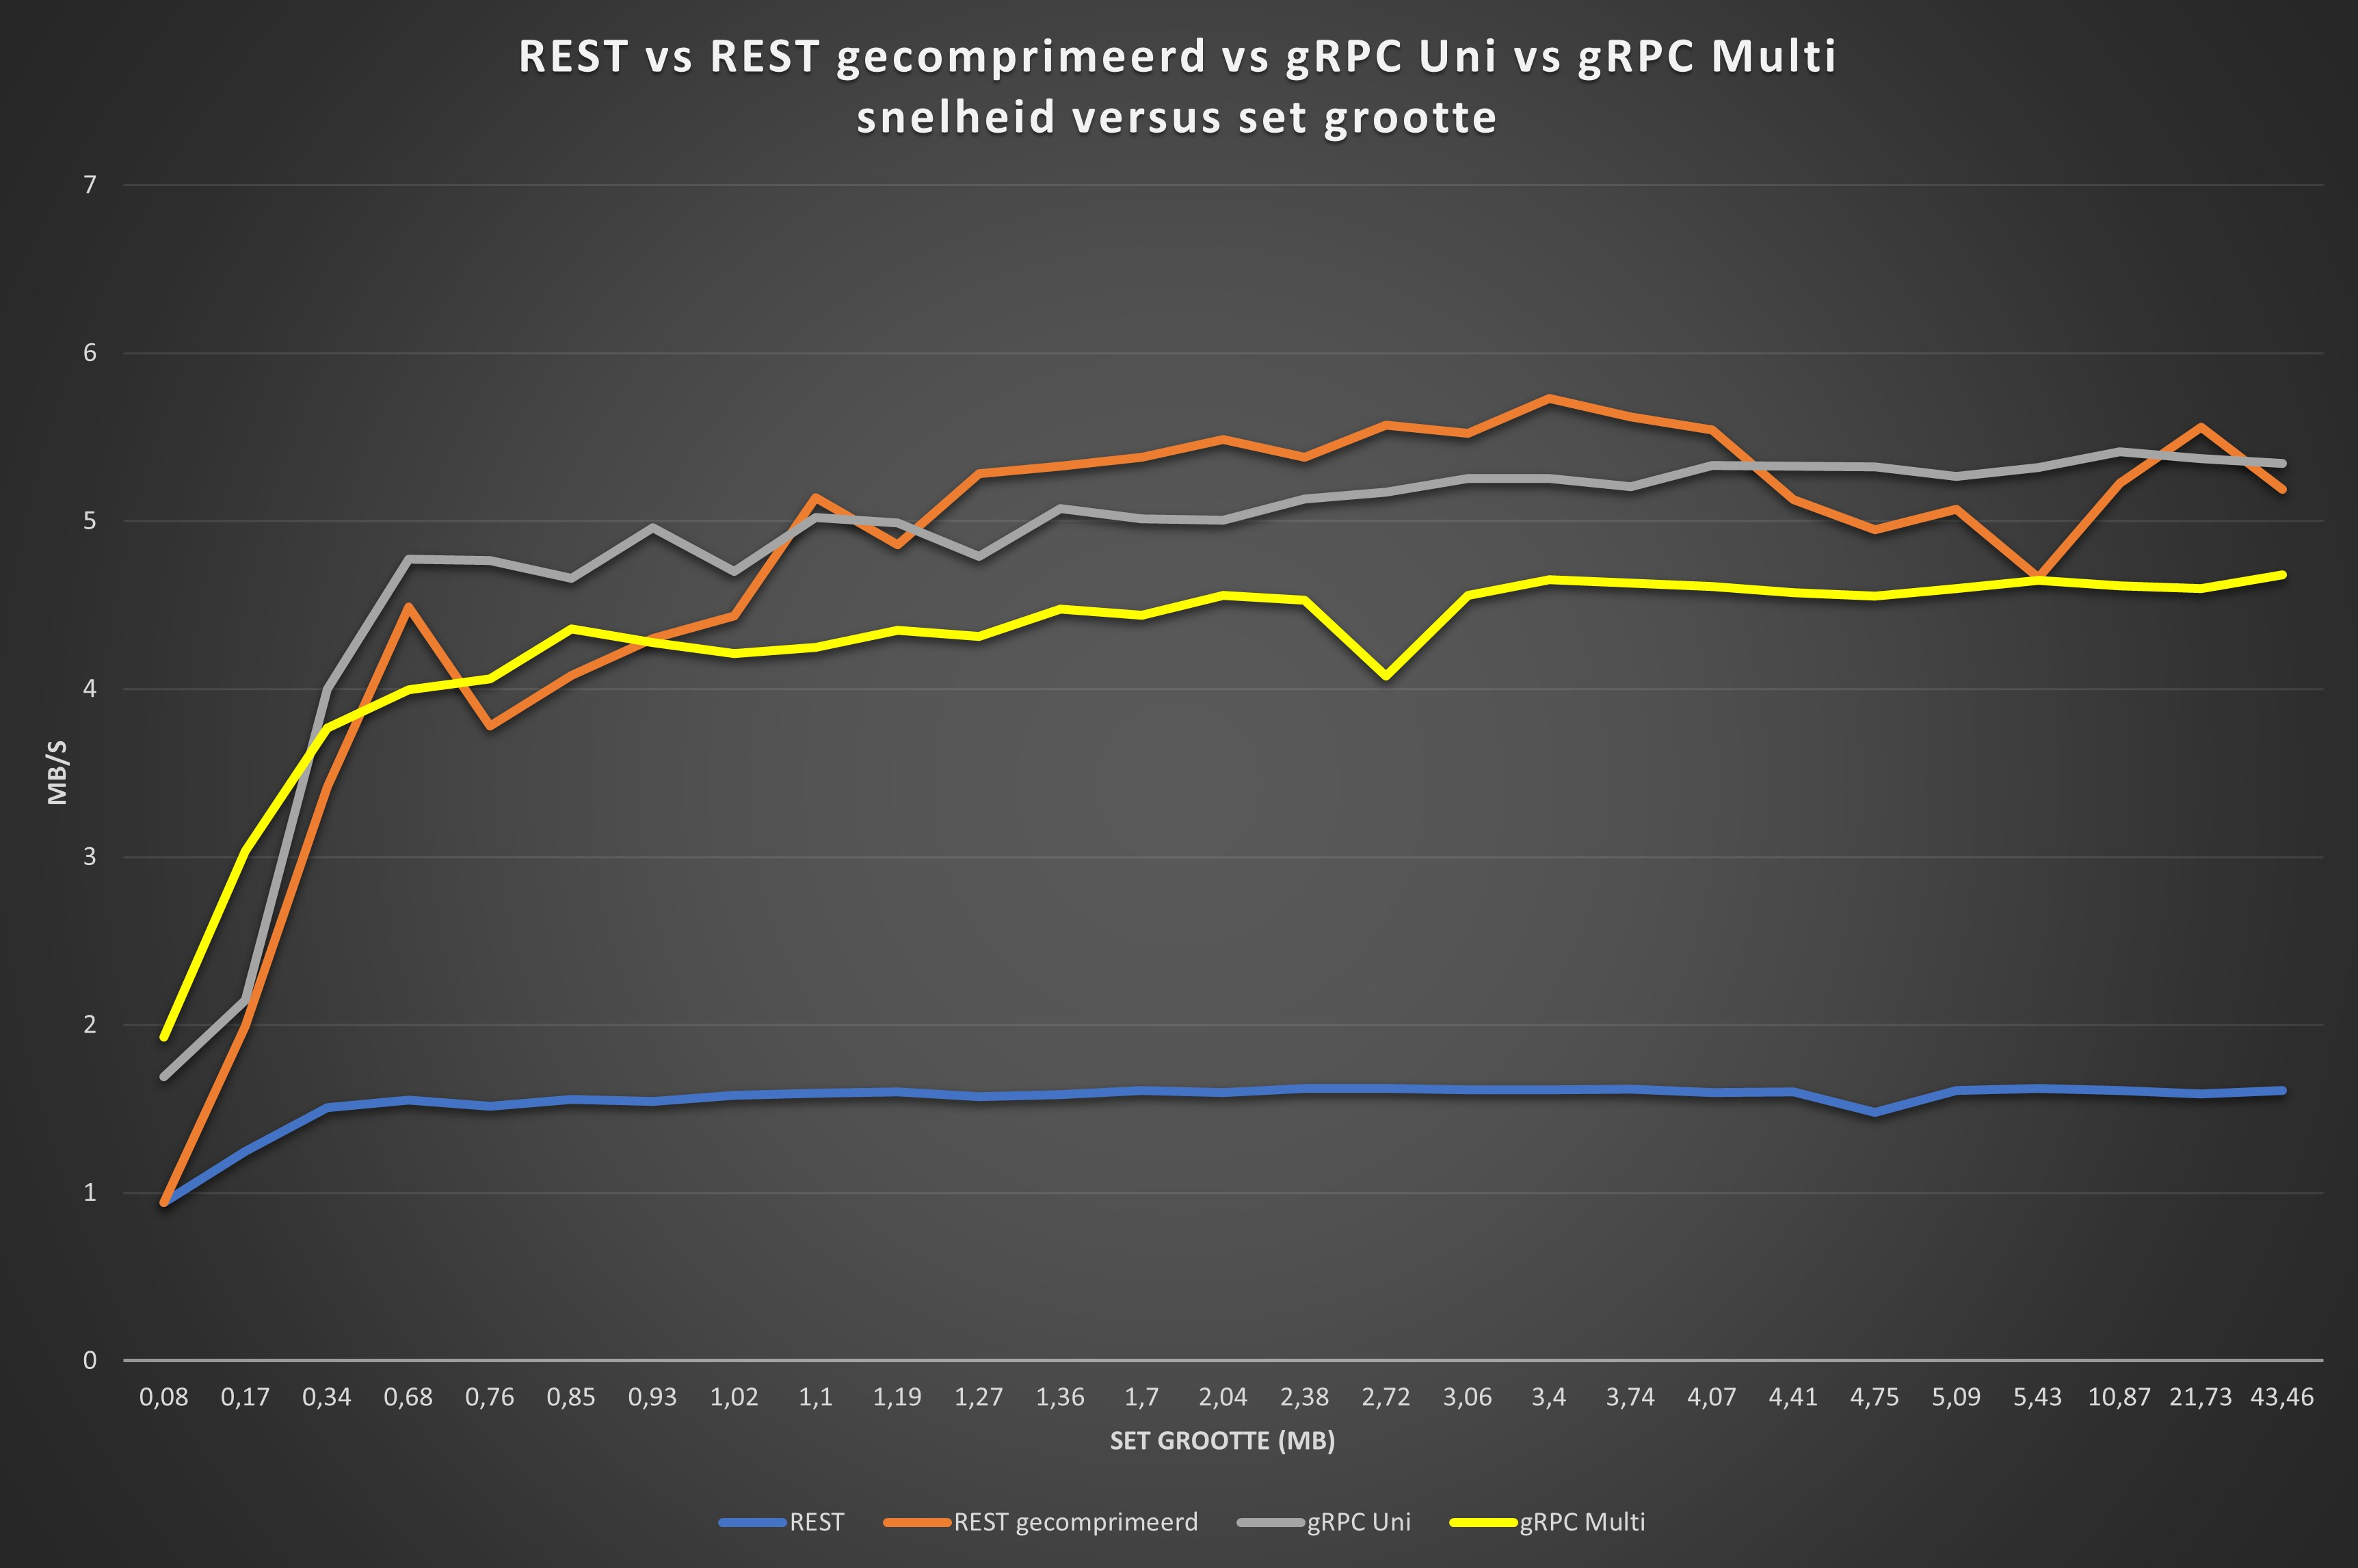
\includegraphics[width=1.0\linewidth]{REST_vs_REST_compressed_vs_gRPC_Uni_vs_gRPC_Multi_singular}
  \caption{REST vs REST met compressie vs gRPC Uni vs gRPC Multi - enkelvoudige requests: snelheid vs. datasets van vari\"erende grootte}
  \label{fig:RESTRESTcompressiegRPCUnigRPCMulti}
\end{center}

\section{Resultaten}

De grafiek in figuur~\ref{fig:RESTRESTcompressiegRPCUnigRPCMulti} toont duidelijk aan dat een standaard REST API met JSON het minst performant is. Echter wanneer het REST API
de data comprimeert alvorens te verzenden is deze juist het meest performante, weliswaar met een kleine marge tegenover gRPC.\\
Wanneer er grotere datasets in stukken verzonden worden en naar de verhouding tussen REST gecomprimeerd en gRPC gekeken wordt valt op dat het REST API met gebruik van compressie
weer het meeste performante is, zie tabel \ref{tab:REST_RESTgecomprimeerd_gRPCUni_gRPCmultimeervoudig} waarbij het tijdsverloop weergegeven wordt van de
meest performante meting voor elk type en dan als percentage t.o.v. het kortste tijdsverloop.\\

\begin{center}
  \begin{tabular}{lllll}
    \toprule
    \textbf{} & \textbf{REST} & \textbf{REST gecomprimeerd} & \textbf{gRPC Uni} & \textbf{gRPC Multi} \\
    \midrule
    tijdsverloop (s) & 214,471 & 59,063 & 65,201 & 73,964 \\
    percentage & 363,12\% & \textbf{100,00\%} & 110,39\% & 125,23\% \\
    \bottomrule
  \end{tabular}
%  \caption{\% tijdsverloop t.o.v. de performantste meting voor grotere datasets in stukken}
  \label{tab:REST_RESTgecomprimeerd_gRPCUni_gRPCmultimeervoudig}
\end{center}

\section{Conclusie}
Het blijkt mogelijk om een REST API ongeveer even performant te maken als een gRPC API. Dan lijkt het belangrijk om bij het overwegen van beide API's voor een nieuwe applicatie
voornamelijk rekening te houden met andere verschillen. Het gegeven dat gRPC niet ondersteund wordt door browsers terwijl dit bij REST zelfs voor compressie het geval is.
REST is zeer wijdverspreid en veelgebruikt terwijl gRPC nog aan het opkomen is.
Voor beide API's is het noodzakelijk om de client te informeren over de werking, het zgn. contract.
Voor REST zijn er op vandaag verschillende mogelijkheden om het API contract bloot te stellen aan clients.
Voor gRPC komt de moeilijkheid van het delen van het .proto bestand daarentegen ook nog aan bod.

\end{multicols}
\end{document}